\section{Knowledge-Guided General Agent Training with Specialized Teachers}
\label{sec:infra}
\subsection{Overview}

\begin{figure}[t]
    \centering
    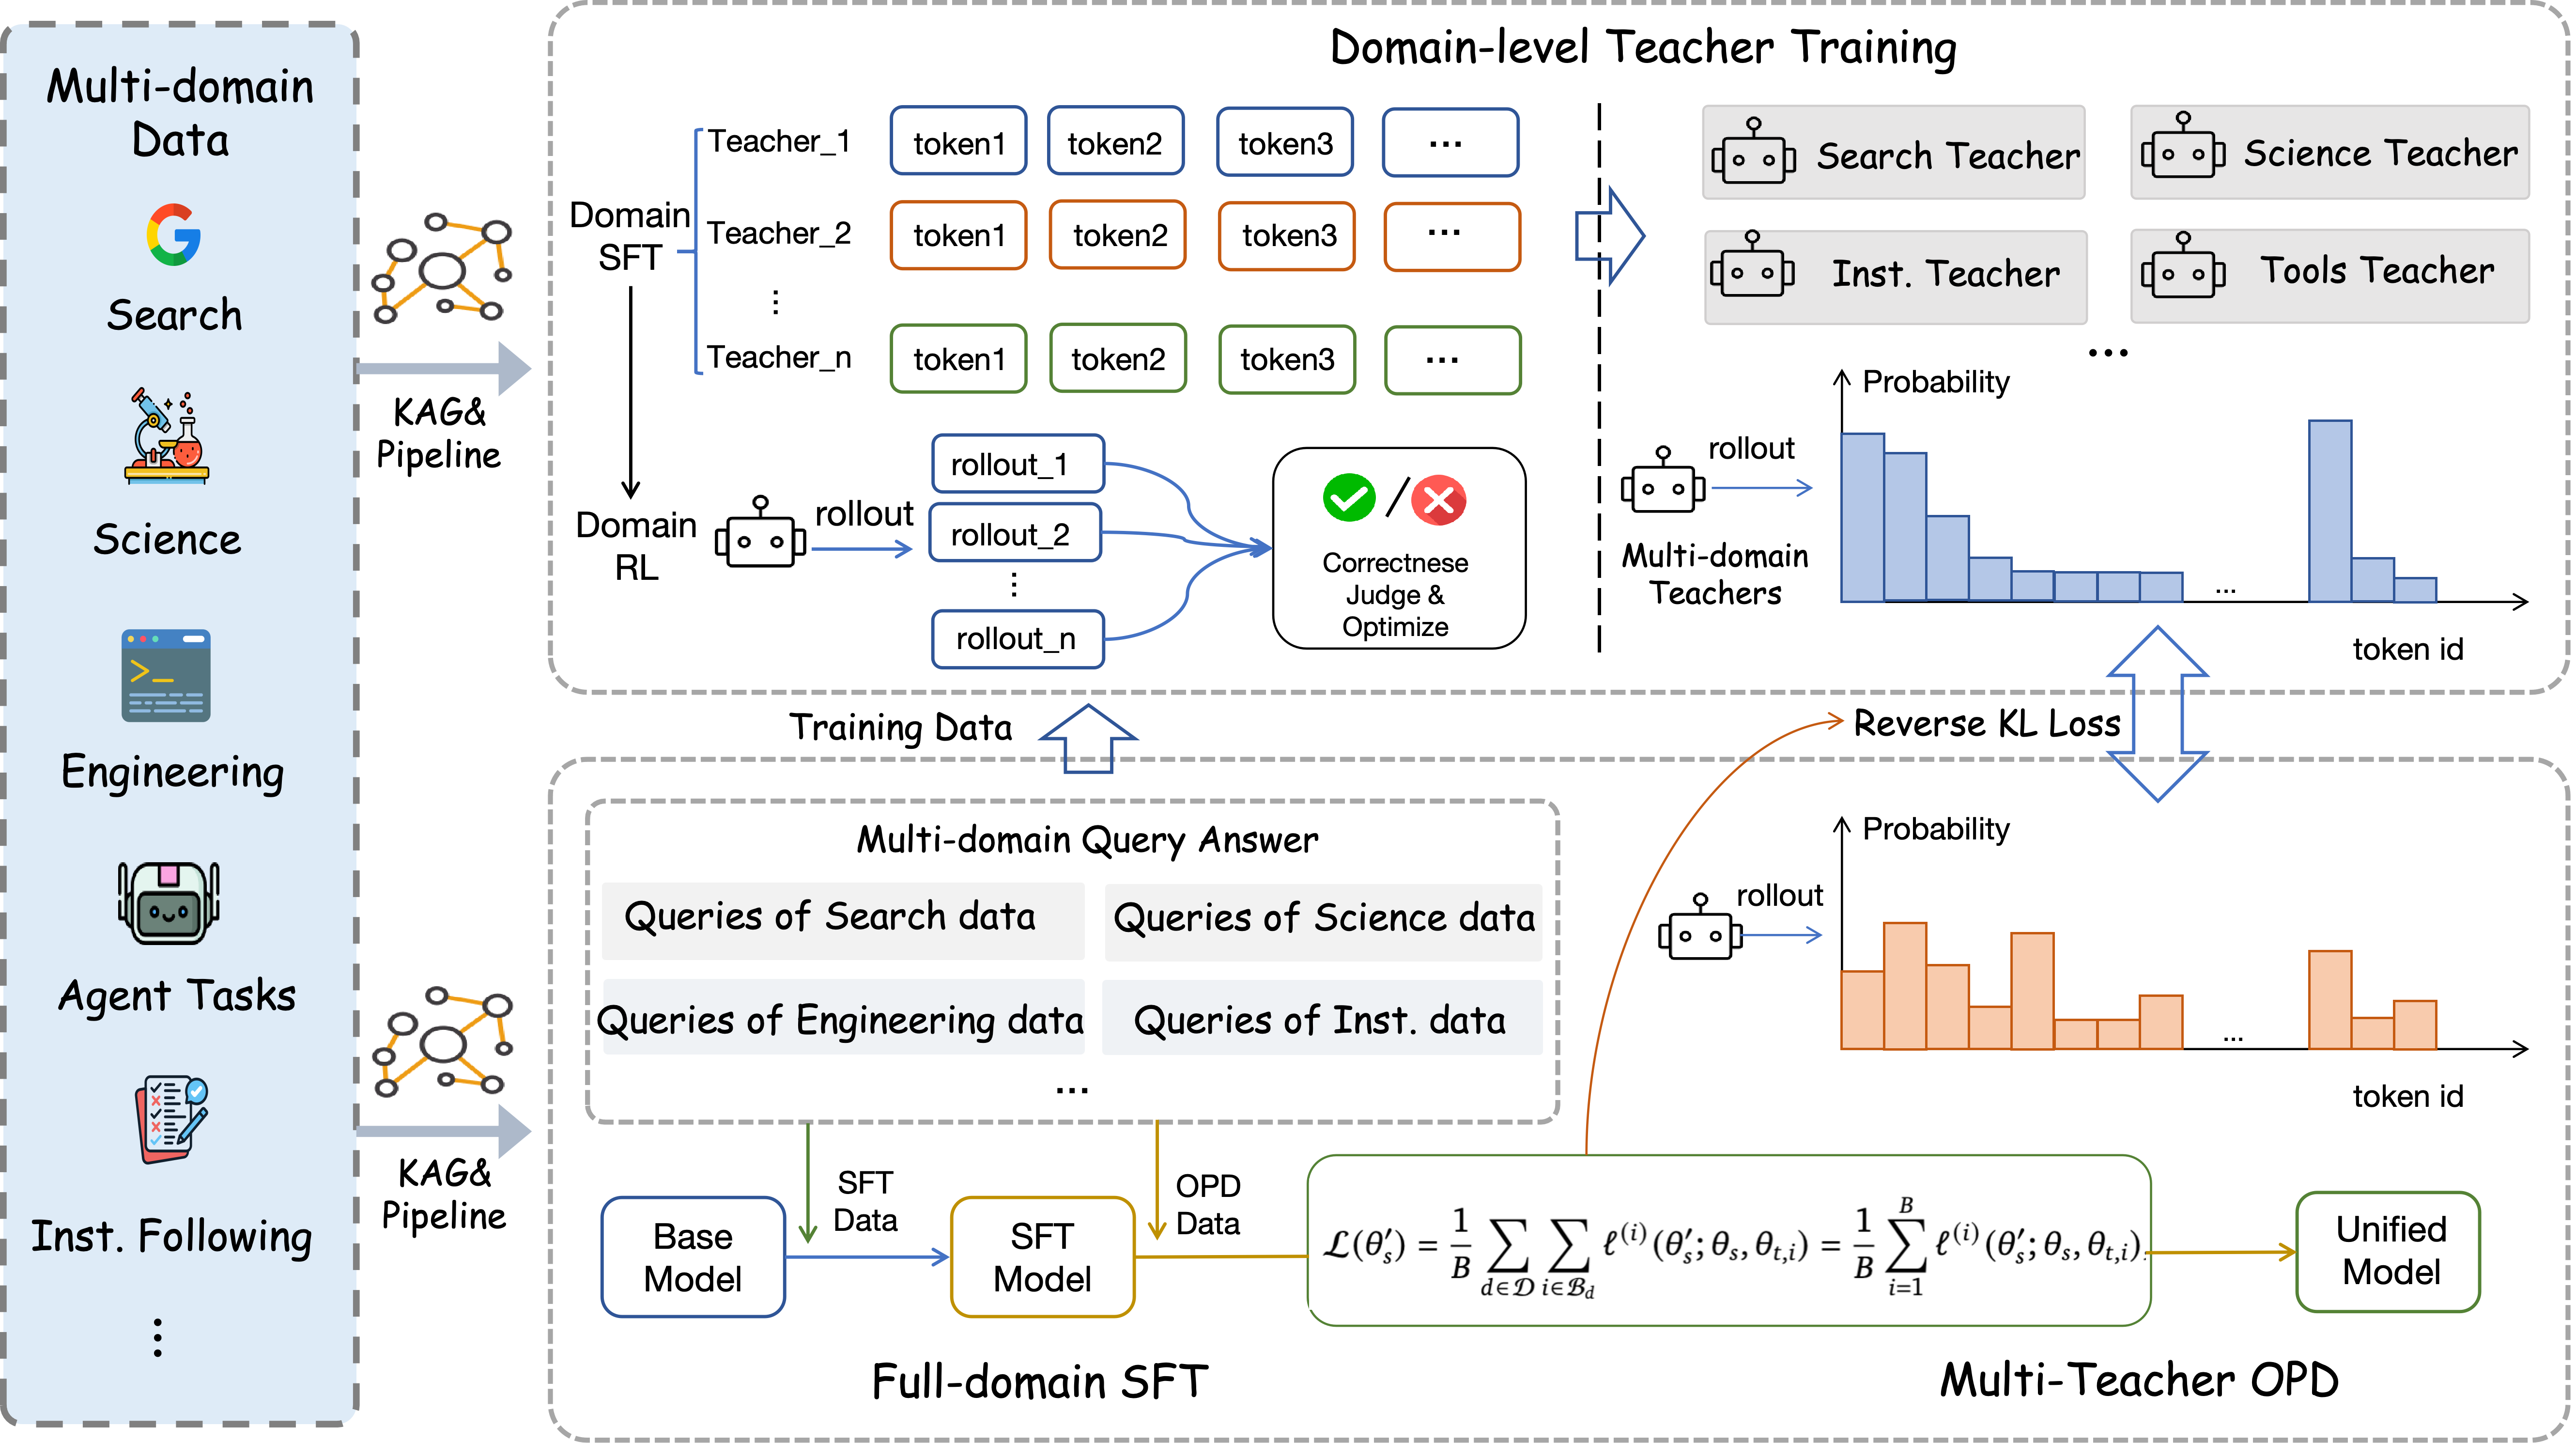
\includegraphics[width=\linewidth]{figures/train_framework.png}
    \caption{Overview of the three-stage training pipeline of \ProjectName. From multi-domain data to domain-specific teachers and multi-teacher on-policy distillation. First, Agents-A1 is trained with full-domain supervised fine-tuning on multi-domain long-horizon data, including search, scientific research, engineering, agentic tasks, and instruction following. Then, domain-specific teacher models are trained on each domain, and their expertise is transferred to the student model through domain-routed on-policy distillation with salient vocabulary alignment.
    }
    \label{fig:training_framework}
\end{figure}

As shown in Figure~\ref{fig:training_framework}, the training process follows a three-stage pipeline. Full-domain supervised fine-tuning is first performed to obtain a broadly capable long-horizon agent. Domain-level teachers are then trained with targeted SFT or RL, enabling each teacher to specialize in a particular capability or interaction pattern. Finally, these teachers are consolidated into a single deployable student through multi-teacher on-policy distillation.

Within this three-stage pipeline, scaling the horizon further depends on both multi-domain data infrastructure and the integration of specialized agent capabilities. For multi-domain data infrastructure, a knowledge-action graph (KAG) is constructed to retain evidence, actions, observations, failures, and verifier outcomes, providing process-level supervision beyond final answers, as described in Sec.~\ref{subsec:knowledge-action-supervision}. For integrating specialized agent capabilities, multi-teacher OPD combines domain teachers into a unified student through routed teacher guidance, salient vocabulary alignment, and domain-aware aggregation, as detailed in Sec.~\ref{subsec:on-policy-distillation}.

%%%%%%%%%%%%%%%%%%%%%%%%%%%%%%%%%%%
\subsection{Long-Horizon Knowledge-Action Infrastructure}
\label{subsec:knowledge-action-supervision}

As LLMs scale, training is increasingly constrained by the availability of high-density, verifiable, and evolvable supervision. Since public web corpora rarely expose provenance, action traces, tool transcripts, execution logs, and verifier outcomes, we construct a knowledge-action infrastructure that converts heterogeneous corpora into compositional, verifiable, and self-extending supervision, as shown in Figure~\ref{fig:kag_infra}.

\begin{figure}[t]
\centering
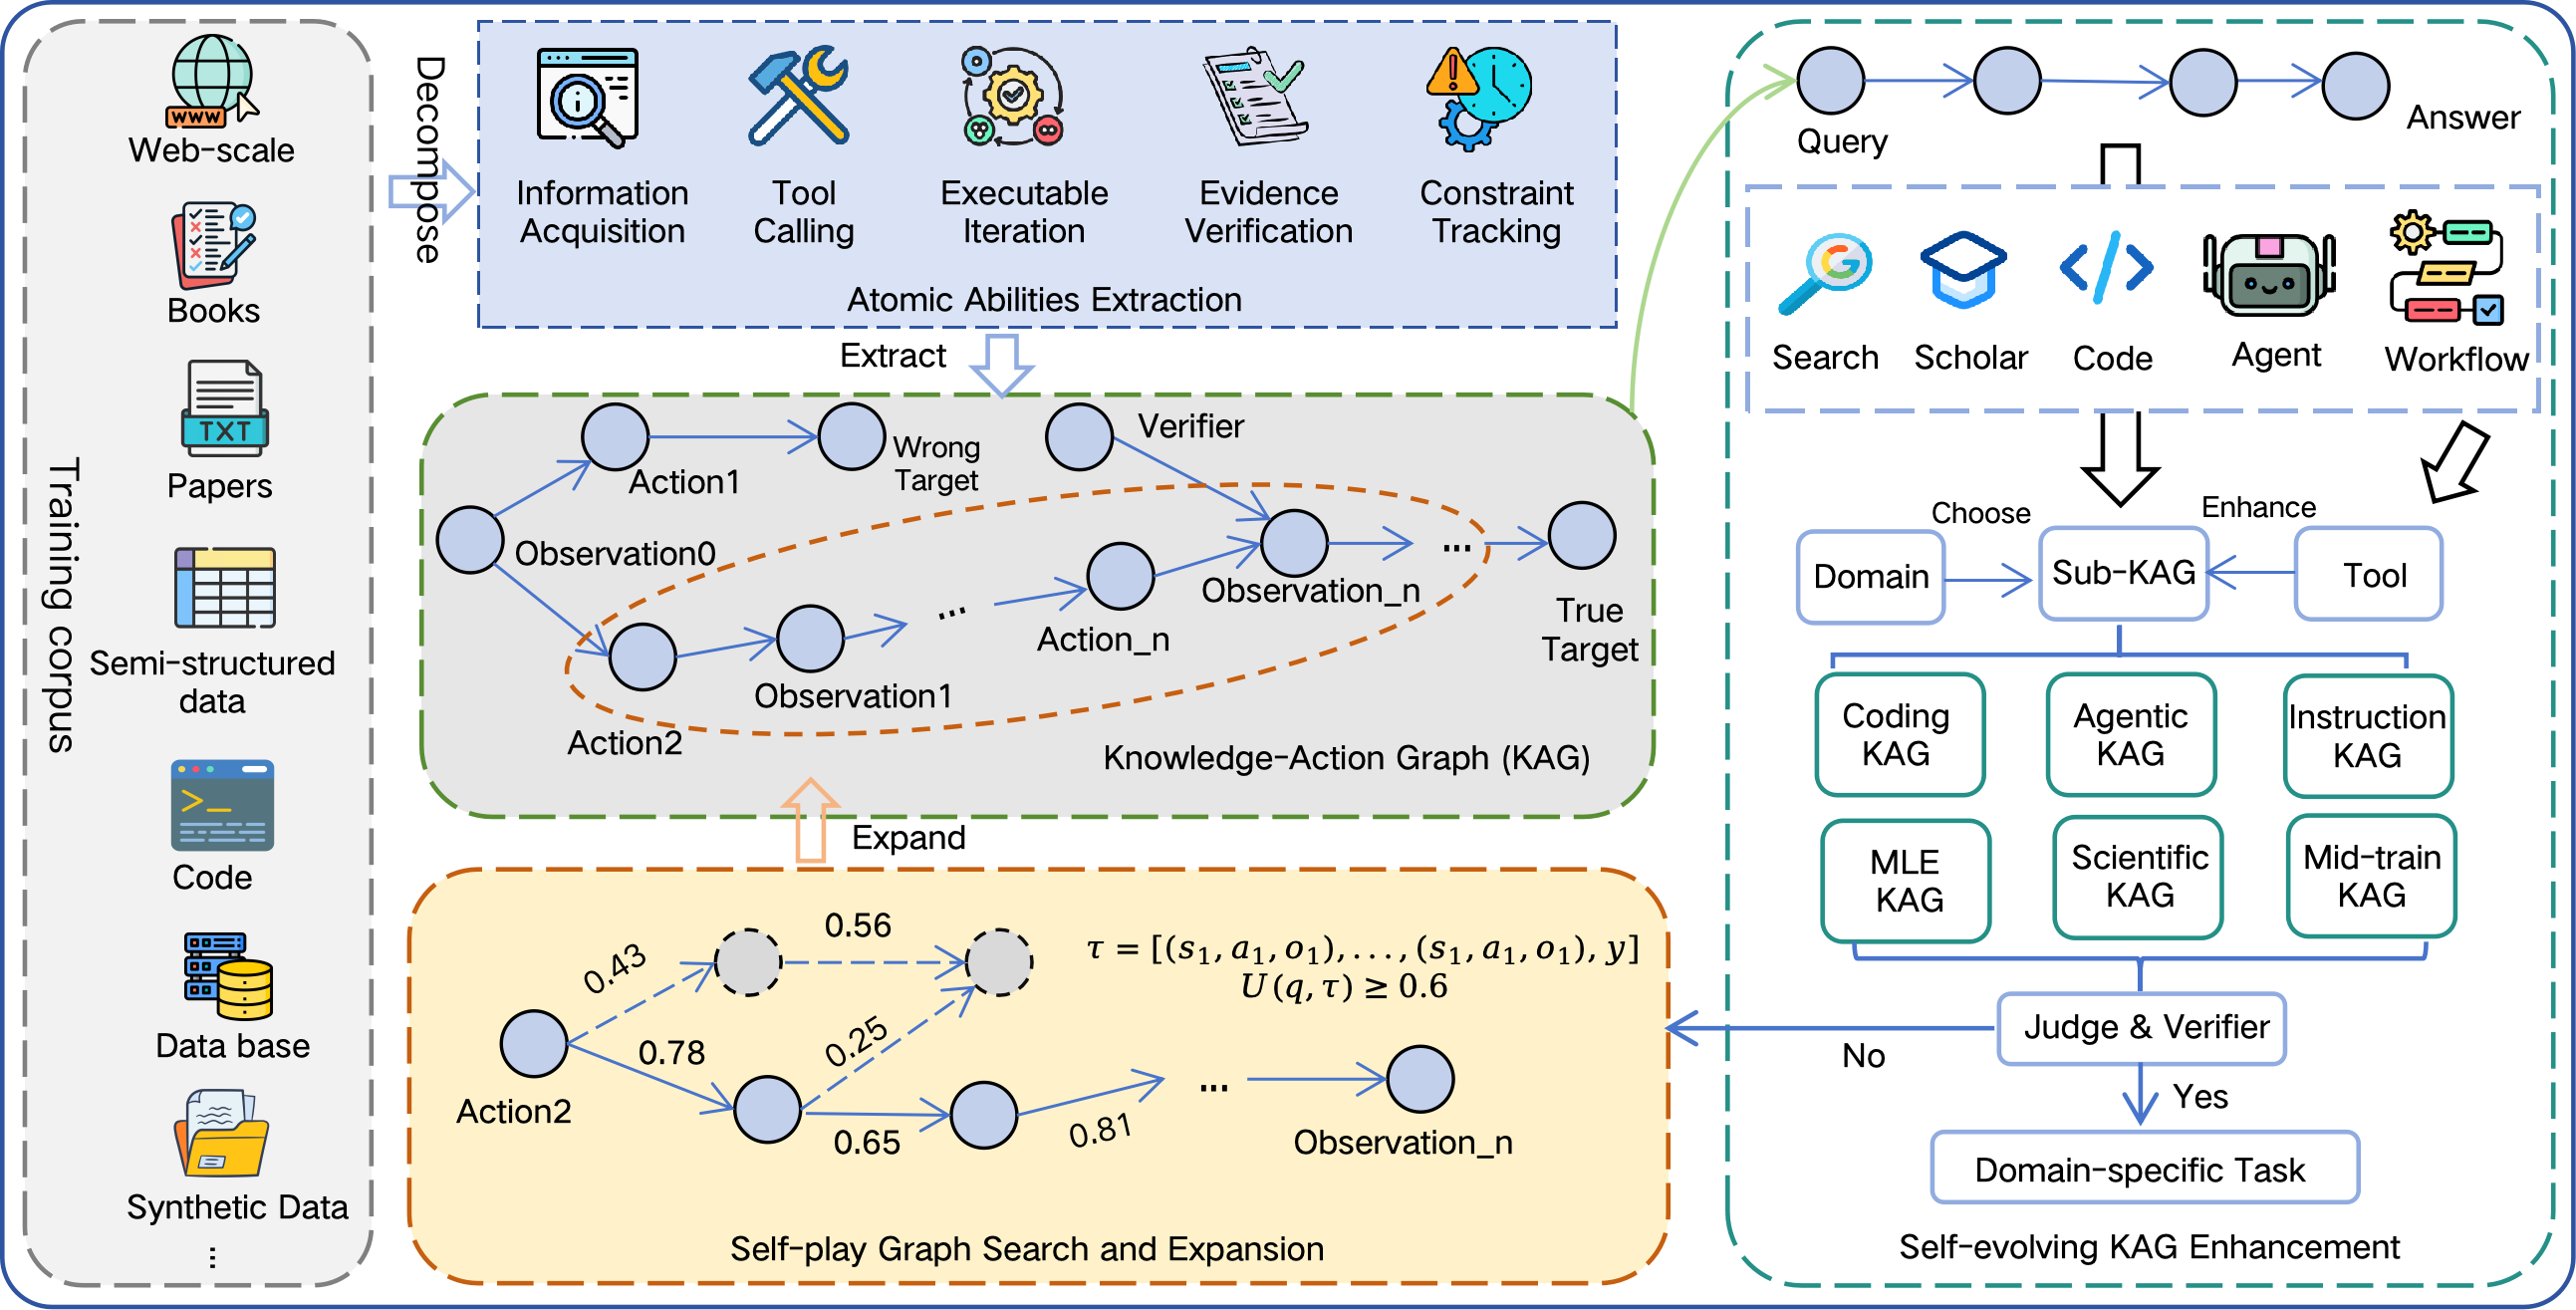
\includegraphics[width=\linewidth]{figures/KAG_infra.png}
\caption{Overview of the knowledge-action infrastructure of \ProjectName. Heterogeneous corpora are decomposed into atomic abilities and organized into a knowledge-action graph (KAG) that records evidence, actions, observations, and verifier outcomes. A tool-augmented self-play loop expands the KAG into domain-specific sub-KAGs for downstream task construction.}
\label{fig:kag_infra}
\end{figure}

\subsubsection{Knowledge-Action Graph Construction with Atomic Abilities}
\label{sec:domain-infrastructure}

We decompose long-horizon agentic competence into five atomic abilities: information acquisition, tool calling, executable iteration, evidence verification, and constraint tracking. To recover supervision for these abilities, we represent evidence, actions, observations, and verifier outcomes as first-class linked objects in a domain-specific knowledge-action graph (KAG). Motivated by previous work~\cite{cao2026agents}, we define the KAG as follows.

\begin{definition}[Knowledge-action graph]
Given a domain $\mathcal{B}_d$ ($d$ denotes the domain), the knowledge-action graph is a typed 4-tuple
\begin{equation}
\mathcal{G}_d = (\mathcal{C}_d,\ \mathcal{A}_d,\ \mathcal{O}_d,\ \mathcal{V}_d),
\label{eq:kag}
\end{equation}
where $\mathcal{C}_d$ is the domain \emph{corpus}, containing evidence chunks, entities, facts, constraints, and other contextual resources of the domain; $\mathcal{A}_d$ is the \emph{action space}, containing tool calls, retrieval queries, code edits and executions, reasoning steps, and other agentic operations available in $\mathcal{B}_d$; $\mathcal{O}_d$ is the \emph{observation space}, containing tool returns, retrieved evidence, execution states, and intermediate artifacts produced by executing actions on $\mathcal{C}_d$; and $\mathcal{V}_d$ is the \emph{verifier set}, containing automatic checks over correctness, evidence support, constraint satisfaction, and goal completion. The graph is populated by linked t-th action records $(s_t, a_t, o_t, v_t)$ with $s_t \subseteq \mathcal{C}_d \cup \mathcal{O}_{<t}$, $a_t \in \mathcal{A}_d$, $o_t \in \mathcal{O}_d$, and $v_t \in \mathcal{V}_d$. Edges between records encode support, dependency, production, verification, and action-transition relations.
\end{definition}

Unlike a conventional knowledge graph that mainly stores entity-relation facts, a KAG preserves the process by which an answer is acquired, tested, revised, and verified through the action records $(s_t, a_t, o_t, v_t)$. This process-level structure retains both successful and failed evidence-backed trajectories, enabling cross-step credit assignment and reproducible long-horizon supervision. 

For example, a long-horizon search task (Section~\ref{sec:search_data}) asks the agent to search an answer entity by navigating hyperlinks through a wiki corpus and web content, where $\mathcal{C}_d$ holds the pages and paragraph evidence, $\mathcal{A}_d$ is the next-hop choice, $\mathcal{O}_d$ the retrieved page text, and $\mathcal{V}_d$ checks whether the answer and its supporting path are recovered. A machine learning engineering task (Section~\ref{sec:mle_data_pipeline}) asks the agent to optimize a Kaggle-style submission by iteratively writing, patching, and executing code over a tree of candidate solution, where $\mathcal{C}_d$ holds the competition specification, dataset, and execution environment, $\mathcal{A}_d$ is a code edit, run, or commit action, $\mathcal{O}_d$ is the resulting log, metric, or submission artifact, and $\mathcal{V}_d$ checks grader scores and submission validity.

\subsubsection{Self-play Graph Search and Expansion}
\label{sec:game-generation}

In practice, the reasoning data generated in a single pass is not necessarily of high quality; it requires multiple iterations and validation to produce.
To optimize and improve the quality of $\mathcal{G}_d$ in each domain, we expand $\mathcal{G}_d$ through a proposer--solver--verifier game: $\pi_{\text{P}}$ samples graph regions to propose constrained tasks, $\pi_{\text{S}}$ solves them with retrieval and tools, and $\pi_{\text{V}}$ verifies answers, evidence, execution results, trajectories, and shortcut risks. Specifically, each generated task is represented as
\begin{equation}
x = (q,\ d,\ \tau,\ y^\star,\ \mathcal{E}_q,\ \mathcal{V}_q),
\qquad
\mathcal{E}_q \subseteq \mathcal{C}_d,\quad \mathcal{V}_q \subseteq \mathcal{V}_d,
\label{eq:task}
\end{equation}
where $q$ is the instruction, $d$ the domain label, $y^\star$ the target answer, $\mathcal{E}_q$ the supporting evidence required for the task, $\mathcal{V}_q$ the verifier subset applicable to the task, and $\tau$ the resulting trajectory
\begin{equation}
\tau = \big[(s_1, a_1, o_1, v_1),\ \ldots,\ (s_T, a_T, o_T, v_T),\ y\big],
\qquad
a_t \in \mathcal{A}_d,\ o_t \in \mathcal{O}_d,\ v_t \in \mathcal{V}_q \cup \{\bot\},
\label{eq:trajectory}
\end{equation}
following the action-record form of Eq.~\ref{eq:kag}, with $v_t = \bot$ when no step-level verifier fires.
A candidate $x$ is accepted by $\pi_{\text{V}}$ only if it is (i) verifiable against some $v \in \mathcal{V}_q$, (ii) valid, i.e., $\tau$ reaches an answer that $v$ accepts, (iii) process-informative, i.e., $\tau$ exercises meaningful intermediate decisions rather than collapsing to a one-shot lookup, (iv) evidence-covering, i.e., the required evidence in $\mathcal{E}_q$ is actually consulted along $\tau$, and (v) unambiguously specified, with no shortcut solution.

In this way, solver and verifier feedback is written back to $\mathcal{G}_d$ as linked states, actions, observations, evidence, artifacts, and verifier outcomes. Given a query-answer pair and an initial KAG, the framework invokes domain tools, including search, scholar, code execution, agent modules, and workflow planners, to enhance the graph. The enhanced graph is specialized into sub-KAGs for coding, agentic reasoning, instruction following, MLE, and scientific reasoning. A judge-and-verifier module accepts qualified sub-KAGs for downstream task-pipeline construction and routes failed ones back to self-play expansion.

%%%%%%%%%%%%%%%%%%%%%%%%%%%%%%%%%%%
\subsection{Domain-Routed On-Policy Distillation with Salient Vocabulary Alignment}
\label{subsec:on-policy-distillation}

Domain-specific teachers provide specialized policies, but deployment requires a single general policy model. Existing sampled-token OPD~\citep{lu2025onpolicydistillation} is efficient because it scores only realized rollout tokens, but this single-token approximation leaves nearby high-probability alternatives unconstrained, a source of unstable or imbalanced guidance noted in recent analyses~\citep{fu2026revisiting,deepseekai2026deepseekv4}.

We therefore use a domain-routed multi-teacher OPD framework with salient vocabulary alignment (SVA). For each prompt-domain pair $(x_i,d_i)$, a frozen rollout student samples $y_i\sim\pi_{\theta_s}(\cdot\mid x_i)$, while the optimized student $\theta_s'$ is supervised by the routed teacher $\theta_{t,i}\triangleq\theta_t^{d_i}$. SVA replaces the sampled-token surrogate by aligning the student and routed teacher on a compact teacher-supported local vocabulary. Losses are computed only on trainable generated tokens $R_i$, with tool outputs and user turns masked out. To handle cross-domain heterogeneity, we aggregate SVA losses with a domain-normalized objective, averaging within each active domain and then across active domains, so that frequent or high-loss domains do not dominate the student update.

\subsubsection{Salient Vocabulary Alignment}

At position $t$, SVA evaluates the current student and the routed teacher on the same student-generated prefix $(x_i,y_{i,<t})$. Let
\[
p_{s'}(u)=\pi_{\theta_s'}(u\mid x_i,y_{i,<t}),
\qquad
p_{t,i}(u)=\pi_{\theta_{t,i}}(u\mid x_i,y_{i,<t}),
\]
and let $\mathcal{S}_{i,t}^{(k)}$ be the set of top-$k$ valid tokens under the routed teacher distribution. We renormalize both distributions on this teacher-selected support
\[
\bar p_{s'}(u)
=
\frac{p_{s'}(u)}
{\sum_{v\in\mathcal{S}_{i,t}^{(k)}}p_{s'}(v)},
\qquad
\bar p_{t,i}(u)
=
\frac{p_{t,i}(u)}
{\sum_{v\in\mathcal{S}_{i,t}^{(k)}}p_{t,i}(v)},
\quad
u\in\mathcal{S}_{i,t}^{(k)}.
\]

The per-sample SVA objective is the truncated reverse KL over this salient support, averaged over trainable model-generated positions
\begin{equation}
\ell_{\mathrm{SVA}}^{(i)}(\theta_s';\theta_{t,i})
=
\frac{1}{|R_i|}
\sum_{t\in R_i}
\sum_{u\in \mathcal{S}_{i,t}^{(k)}}
\bar p_{s'}(u)
\log
\frac{\bar p_{s'}(u)}{\bar p_{t,i}(u)} .
\end{equation}

Because the support is teacher-selected, SVA does not directly constrain student mass outside $\mathcal{S}_{i,t}^{(k)}$. We therefore monitor the student-side coverage
\begin{equation}
\rho(i,t)
=
\sum_{u\in \mathcal{S}_{i,t}^{(k)}} p_{s'}(u),
\end{equation}
where higher coverage indicates a closer approximation to full-vocabulary alignment.


\subsubsection{Domain-routed Normalized Objective}

In the multi-domain setting, different domains may induce heterogeneous gradients because they emphasize different capabilities, such as response style, reasoning pattern, evidence acquisition, tool use, or external interaction. We use hard domain routing, where each sample is supervised only by the teacher trained for its domain,
\[
\theta_{t,i} = \theta_t^{d_i},
\]
rather than by a soft mixture of teachers. This preserves domain-specific teacher preferences and avoids mixing incompatible teacher signals at the token level.

For a mini-batch $\mathcal{B}$, let $\mathcal{B}_d$ denote the subset of samples from domain $d$, and let
\[
\mathcal{D}_{\mathcal{B}}
=
\{d\in\mathcal{D}\mid |\mathcal{B}_d|>0\},
\]
be the set of active domains. Since each per-sample SVA loss is already averaged over its own trainable response positions, longer trajectories do not dominate merely by contributing more tokens. To further prevent high-frequency domains from dominating the update, we average losses within each active domain and then average over active domains:
\begin{equation}
\mathcal{L}_{\mathrm{MT\text{-}SVA}}(\theta_s')
=
\frac{1}{|\mathcal{D}_{\mathcal{B}}|}
\sum_{d\in \mathcal{D}_{\mathcal{B}}}
\frac{1}{|\mathcal{B}_d|}
\sum_{i\in \mathcal{B}_d}
\ell_{\mathrm{SVA}}^{(i)}(\theta_s';\theta_{t,i}).
\end{equation}
This domain-normalized objective gives each active domain comparable influence while allowing each sample to receive supervision from its corresponding domain-specific teacher. Domain labels are also used to instantiate domain-specific rollout protocols, such as finalization rules, simulated user turns, or environment-specific tool execution. After rollouts are generated, all trainable positions are optimized using the same SVA objective under their routed teachers.
